\documentclass{if-beamer}

% --------------------------------------------------- %
%                  Presentation info	              %
% --------------------------------------------------- %
\title[Lecture 9]{Lecture 9}
\subtitle{Using Pointers}
\author{Instructor: Ashley Gannon}
\date{ISC3313 Fall 2021}
\logo{
\includegraphics[scale=0.08]{figures/FSULogo.png}
}
\subject{Presentation subject}

\lstset{language=C++,
	basicstyle=\ttfamily,
	keywordstyle=\color{blue}\ttfamily,
	stringstyle=\color{red}\ttfamily,
	commentstyle=\color{green}\ttfamily,
	morecomment=[l][\color{magenta}]{\#}
}
% --------------------------------------------------- %
%                    Title + Schedule                 %
% --------------------------------------------------- %

\begin{document}
	
\begin{frame}
	\titlepage
\end{frame}

% --------------------------------------------------- %
%                      Presentation                   %
% --------------------------------------------------- %

\begin{frame}[fragile]
\frametitle{Pointers to arrays}
Last class we saw how to use a pointer to a chunk of memory. This is known as
\textit{dynamic} memory.
\begin{lstlisting}
int n = 10;
int* p = new int[n];
for (int i = 0; i < 10; i++)
{
p[i] = i;
}
cout<<*p;
\end{lstlisting}
\end{frame}

\begin{frame}[fragile]
\frametitle{Pointers to arrays}
Last class we saw how to use a pointer to a chunk of memory. This is known as
\textit{dynamic} memory.
\begin{lstlisting}
int n = 10;
int* p = new int[n];
for (int i = 0; i < 10; i++)
{
p[i] = i;
}
cout<<p[4];
\end{lstlisting}
\end{frame}

\begin{frame}[fragile]
\frametitle{Pointers to arrays}
Last class we saw how to use a pointer to a chunk of memory. This is known as
\textit{dynamic} memory.
\begin{lstlisting}
int n = 10;
int* p = new int[n];
for (int i = 0; i < 10; i++)
{
p[i] = i;
}
cout<<*p[4];
\end{lstlisting}
\end{frame}

\begin{frame}[fragile]
\frametitle{Pointers to arrays: deleting the heap}
Delete can be used by either using \texttt{Delete operator} or \texttt{Delete [] operator} \\
\vspace{5pt}
Using \texttt{new} for dynamic memory allocation puts variables on heap memory. Which means Delete operator deallocates memory from heap.\\
\vspace{5pt}
NOTE: The pointer to object is not destroyed, value or memory block pointed by pointer is available to reuse.

\begin{lstlisting}
int n = 10;
int* p = new int[n];
for (int i = 0; i < 10; i++)
{
p[i] = i;
}
delete[] p;
\end{lstlisting}
\end{frame}

\begin{frame}
\frametitle{Discretization}
\textbf{Discretization} is the process of transferring continuous functions, models, variables, and/or equations into discrete counterparts. This process is usually carried out as a first step toward making them suitable for numerical evaluation.\\
\vspace{5pt}
Let's consider the continuous variable $x$, that exists on the domain $[0,4]$. 

\begin{figure}
	\centering
	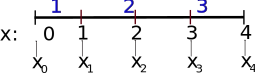
\includegraphics[width = .8\textwidth]{figures/space1}
\end{figure}
\end{frame} 

\begin{frame}
\frametitle{Discretization}
\textbf{Discretization} is the process of transferring continuous functions, models, variables, and/or equations into discrete counterparts. This process is usually carried out as a first step toward making them suitable for numerical evaluation.\\
\vspace{5pt}
Let's consider the continuous variable $x$, that exists on the domain $[0,4]$. \\
\begin{itemize}
	\item We want to discretize this domain by chopping it into 4 parts.
\end{itemize}

\begin{figure}
	\centering
	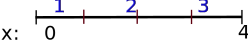
\includegraphics[width = .8\textwidth]{figures/space2}
\end{figure}
\end{frame} 

\begin{frame}
\frametitle{Discretization}
\textbf{Discretization} is the process of transferring continuous functions, models, variables, and/or equations into discrete counterparts. This process is usually carried out as a first step toward making them suitable for numerical evaluation.\\
\vspace{5pt}
Let's consider the continuous variable $x$, that exists on the domain $[0,4]$. \\
\begin{itemize}
	\item We want to discretize this domain by chopping it into 4 parts.
	\item Set the values of x
\end{itemize}

\begin{figure}
	\centering
	\includegraphics[width = .8\textwidth]{figures/space3}
\end{figure}
\end{frame} 

\begin{frame}
\frametitle{Discretization}
\textbf{Discretization} is the process of transferring continuous functions, models, variables, and/or equations into discrete counterparts. This process is usually carried out as a first step toward making them suitable for numerical evaluation.\\
\vspace{5pt}
Let's consider the continuous variable $x$, that exists on the domain $[0,4]$. \\
\begin{itemize}
	\item We want to discretize this domain by chopping it into 4 elements (parts).
	\item Set the values of x\\
\end{itemize}

\begin{figure}
	\centering
	\includegraphics[width = .8\textwidth]{figures/space4}
\end{figure}

\vspace{5pt}
NOTICE: we have 4 elements, but 5 points in our array. 
\end{frame} 

\begin{frame}[fragile]
\frametitle{Class activity 1}
We are going to discretize a domain $x \in [x_a,x_b]$ by chopping it into $N$
separate elements. Each element will be of size
\begin{equation*}
\Delta x = \frac{x_b - x_a}{N}
\end{equation*}
There will be $N+1$ points. We are going to store them in an array. For
integer $i$ is 0 to $N$ we need to compute
\begin{equation*}
x_{i} = i * \Delta x
\end{equation*}
Let $x_a = 0$, $x_b = 20$, and $N = 20$. Compute $\Delta x$ once and store it. Then use a \texttt{for} loop to compute the $x_{i}$. Print out x to verify your code is correct.\\

\vspace{10pt}
Post your code in the discussion board \textbf{Discretization Code} for participation credit.
\end{frame}

\begin{frame}[fragile]
\frametitle{Pointers for passing arrays}
We saw how to pass a variable to a function by reference. It is possible to
do this using pointers as well.
\begin{lstlisting}
int n = 10;
int* p = new int[n];
myfunc(p,n);
\end{lstlisting}
where the declaration of \texttt{myfunc} might look like:
\begin{lstlisting}
void myfunc(int* a, int N);
\end{lstlisting}
\end{frame}

\begin{frame}[fragile]
\frametitle{Class activity 2}
Write a \texttt{void} function (called \texttt{linspace}) that takes as an
argument \\
\vspace{5pt}
\begin{itemize}
	\item a pointer (type \texttt{double}),\\
	\item lower and upper bounds ($x_a$ and $x_b$, type \texttt{double}), \\
	\item and the number of elements ($N$ type \texttt{int}) for the domain
	to be discretized by	\\
\end{itemize}
\vspace{5pt}
The code should compute $N+1$ points along the domain and store them in the array pointer. Test your code for $N = 10$, and $x_a = 0$, $x_b = 1$.\\

\vspace{10pt}
Post your code in the discussion board \textbf{Linspace Function} for participation credit.
\end{frame}


\end{document}
